\documentclass[12pt]{article}
\usepackage[a4paper,margin=1in]{geometry}
\usepackage{hyperref}
\usepackage{longtable}
\usepackage{graphicx}
\usepackage{amsmath}
\usepackage{booktabs}
\usepackage[utf8]{inputenc}
\usepackage{tabularx} % Required for word wrapping and width control
\usepackage{makecell} % Optional, but good for extra formatting
\usepackage{float}
\hypersetup{
    colorlinks=true,
    linkcolor=cyan,
    urlcolor=blue,
    citecolor=black
}


\begin{document}

% --- START OF COVER PAGE ---
\begin{titlepage}
    \flushright % Aligns everything to the right to match image_a197df.png
    
    \vspace*{0.05in}
    
    \vspace{1in}
    
    % Main Title
    {\Huge \textbf{Software Metrics \&}} \\[0.2cm]
    {\Huge \textbf{Risk Handling}} \\
    
    \vspace{0.8in}
    
    {\Large \textbf{for}} \\
    
    \vspace{0.8in}
    
    % Product Name
    {\Huge \textbf{MiniOS Design}} \\
    
    \vfill % Pushes the following content to the bottom
    
    \vspace{1in}
    
    {\large \textbf{Prepared by Group - 2}} \\
    
    \vspace{0.8in}
    
    % Team Members Block
    {\large Group 2 Members :} \\
    {\large Aditya Sharma (B24CS1119)} \\
    {\large Mehta Taksh Ashish (B24CS1115)} \\
    {\large Ved Mitra Verma (B24CS1086)} \\
    {\large Mayank Tiwari (B24CS1098)} \\
    
    \vspace{1in}
    
    % Date
    {\large \textbf{03-04-2026}}
    
\end{titlepage}

%------END of cover page------%

\newpage
\tableofcontents
\newpage

\section{Section - I}

\textbf{Codebase Size Configuration:}
\begin{itemize}
    \item Extracted Added/Modified Lines from xv6 Base: 41,424
    \item Applied Reuse Factor: 5\% (Given xv6 is a heavily reused existing codebase)
    \item \textbf{Effective Lines of Code (LOC): 2,071 (KLOC = 2.071)}
\end{itemize}
\textit{Note: This adaptation factor correctly aligns the metrics to represent a realistic effort constraint for a 4-person team over a 4-month semester limits.}
\vspace{0.3cm}

\subsection{Intermediate COCOMO}
The Constructive Cost Model (COCOMO) estimates the required effort and schedule. The ``Organic'' mode was selected, mapping to small projects with small, familiar teams.

\textbf{Factors Used:}
\begin{itemize}
    \item Scale Factors: $a_b = 3.2$, $b_b = 1.05$, $c_b = 2.5$, $d_b = 0.38$
    \item Effort Adjustment Factor (EAF): $1.2035$ (Derived from Reliability=1.15, Complexity=1.15, Tool Use=0.91)
\end{itemize}

\textbf{Calculated Results:}
\begin{itemize}
    \item \textbf{Effort}: 8.27 Person-Months
    \item \textbf{Development Time}: 5.58 Months
    \item \textbf{Team Size Required}: 1.48 Developers
\end{itemize}

\subsection{Halstead Metric}
Halstead measures complexity mathematically based on discrete operators and operands distributed logically recursively across core C files.

\textbf{Formulas Used:}
\begin{itemize}
    \item Vocabulary ($n$) $= n_1 + n_2$
    \item Length ($N$) $= N_1 + N_2$
    \item Volume ($V$) $= N \times \log_2(n)$
    \item Difficulty ($D$) $= (n_1/2) \times (N_2/n_2)$
    \item Effort ($E$) $= D \times V$
\end{itemize}

\textbf{Extracted Parameters:}
\begin{itemize}
    \item Unique Operators ($n_1$): 13 \textit{(e.g., -, for, else, while, return, if, <, =, *, !, >, /, +)}
    \item Total Operators ($N_1$): 3263
    \item Unique Operands ($n_2$): 851
    \item Total Operands ($N_2$): 7319
\end{itemize}

\textbf{Calculated Results:}
\begin{itemize}
    \item \textbf{Vocabulary ($n$)}: 864
    \item \textbf{Length ($N$)}: 10582
    \item \textbf{Volume ($V$)}: 103,226.22
    \item \textbf{Difficulty ($D$)}: 55.90
    \item \textbf{Effort ($E$)}: 5,770,661.05
\end{itemize}

\subsection{Function Point Analysis}
Function Point Analysis calculates functional software size derived from logic representations.

\textbf{Factors \& Formulas Used:}
\begin{itemize}
    \item Weight Adjustments: Internal Logical File (ILF) Weight = 7, External Input (EI) Weight = 4
    \item Value Adjustment Factor (VAF) $= 0.65 + (0.01 \times 14 \times 3) = 1.07$
\end{itemize}

\textbf{Extracted Parameters:}
\begin{itemize}
    \item Internal Logical Files (Structs identified): 113
    \item External Inputs/Outputs (Syscalls identified): 143
\end{itemize}

\textbf{Calculated Results:}
\begin{itemize}
    \item \textbf{Unadjusted Function Points (UFP)}: 1363
    \item \textbf{Function Points (FPA)}: 1458.41
\end{itemize}

\subsection{Cumulative Flow Diagram}
The Cumulative Flow Diagram (CFD) visualizes task aggregation throughout the project lifecycle against the baseline capacity requirements.
\begin{figure}[H]
    \centering
    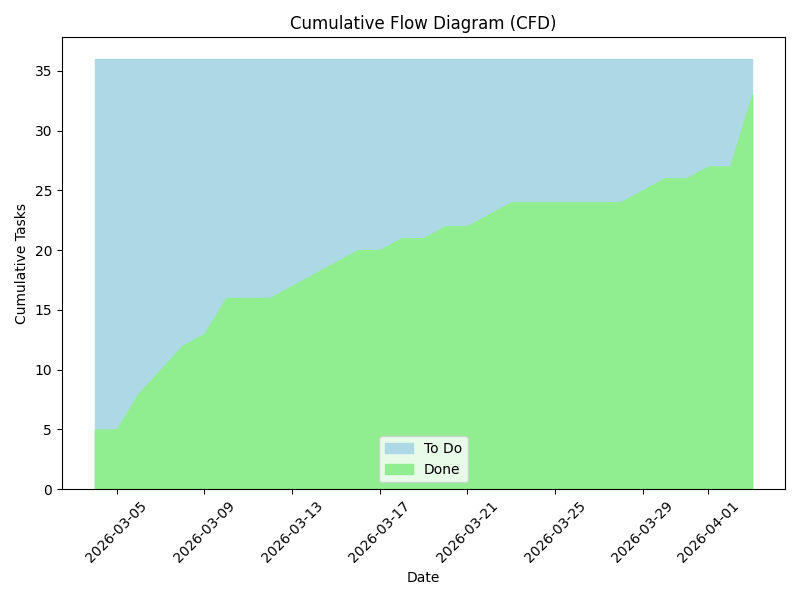
\includegraphics[width=0.85\textwidth]{agile_cfd.png}
    \caption{Cumulative Flow Diagram}
\end{figure}

\subsection{Throughput Report}
The Throughput report identifies timeline velocity mapping precisely when issues were migrated successfully from 'In-Progress' to 'Done'.
\begin{figure}[H]
    \centering
    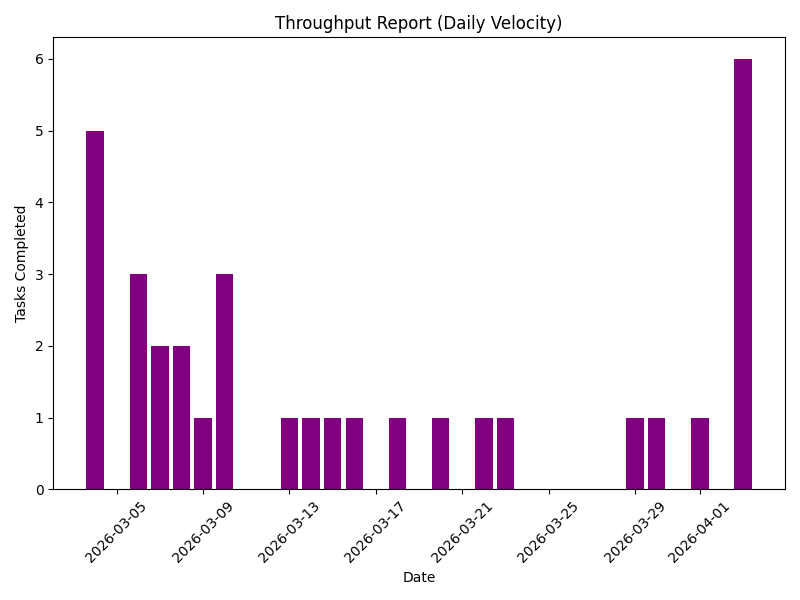
\includegraphics[width=0.85\textwidth]{agile_throughput.png}
    \caption{Throughput Report (Daily Velocity)}
\end{figure}

\subsection{Sprint Burndown Chart}
The Sprint Burndown captures daily sprint variance of open items falling recursively toward an ideal targeted schedule.
\begin{figure}[H]
    \centering
    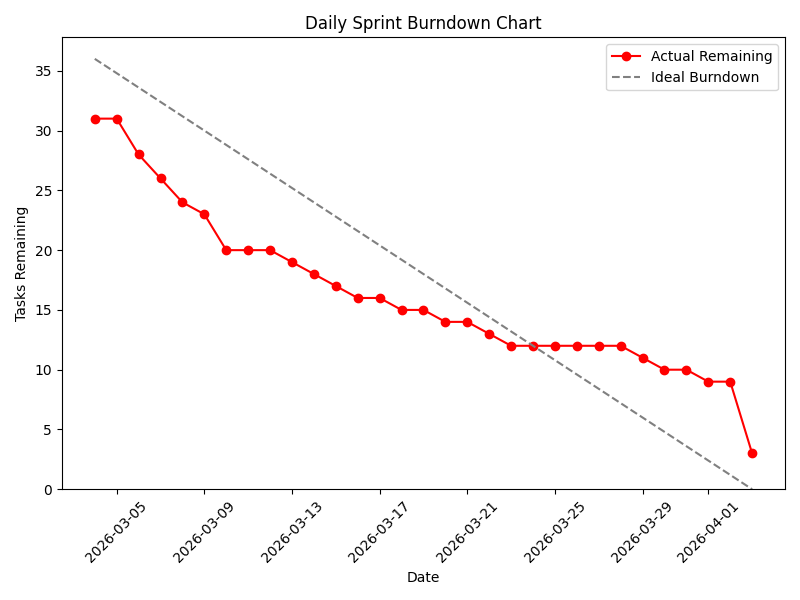
\includegraphics[width=0.85\textwidth]{agile_burndown_chart.png}
    \caption{Daily Sprint Burndown Chart}
\end{figure}

\subsection{Sprint Burnup Chart}
Our Burnup highlights accumulative achievements ascending continuously toward total scope delivery.
\begin{figure}[H]
    \centering
    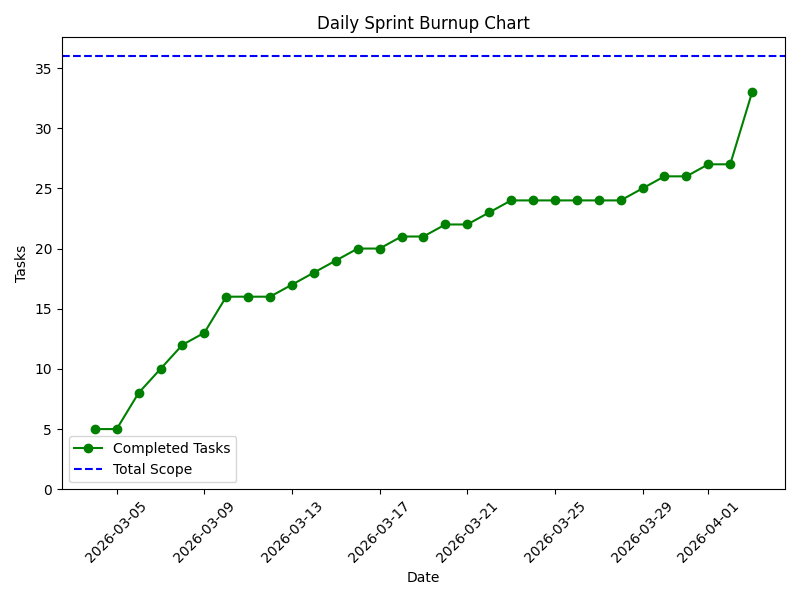
\includegraphics[width=0.85\textwidth]{agile_burnup_chart.png}
    \caption{Daily Sprint Burnup Chart}
\end{figure}

\subsection{Any 2 Metrics}

\subsubsection{1. ABC Metric (Assignment-Branch-Condition)}
The ABC framework evaluates complexity through dimensions representing internal logical flow boundaries.
\begin{itemize}
    \item \textbf{Formula Used}: $ABC\ Magnitude = \sqrt{A^2 + B^2 + C^2}$
    \item Assignments ($A$): 458
    \item Branches ($B$): 256
    \item Conditions ($C$): 705
    \item \textbf{ABC Magnitude}: 878.82
\end{itemize}

\subsubsection{2. Cyclomatic Complexity (V(G))}
Cyclomatic complexity offers a quantitative tracking path mechanism for identifying non-linear control logic structures routing.
\begin{itemize}
    \item \textbf{Formula Used}: $V(G) = \text{Edges} - \text{Nodes} + 2$ (Simplified functionally as: Branches + Conditions + 1 per logic flow)
    \item \textbf{Total Nodes (N)}: 1544
    \item \textbf{Total Edges (E)}: 1896
    \item \textbf{Total V(G) Index metric}: 372
\end{itemize}

\newpage
\section{Section - II}


\section{Section - III}


\end{document}